%%%%%%%%%%%%%%%%%%%%%%%%%%%%%%%%%%%%%%%%%%%%%
% PROCESAMIENTO DIGITAL DE SEÑALES DE AUDIO
% MAESTRÍA EN INGENIERÍA ELÉCTRICA, UDELAR
% SEGUNDO SEMESTRE 2016
%%%%%%%%%%%%%%%%%%%%%%%%%%%%%%%%%%%%%%%%%%%%%

%----------------------------------------------------------------------------------------
%	PACKAGES AND DOCUMENT CONFIGURATIONS
%----------------------------------------------------------------------------------------

\documentclass{article}

\usepackage[version=3]{mhchem} % Package for chemical equation typesetting
\usepackage{siunitx} % Provides the \SI{}{} and \si{} command for typesetting SI units

\usepackage[spanish]{babel}
\selectlanguage{spanish}
\usepackage[utf8]{inputenc}
\usepackage{graphicx} % Required for the inclusion of images
\usepackage{natbib} % Required to change bibliography style to APA
\usepackage{amsmath} % Required for some math elements 

\usepackage{float}

\usepackage{geometry}
 \geometry{
 a4paper,
 total={170mm,257mm},
 left=20mm,
 top=20mm,
 }

\usepackage{listings}
\usepackage{color} %red, green, blue, yellow, cyan, magenta, black, white
\definecolor{mygreen}{RGB}{28,172,0} % color values Red, Green, Blue
\definecolor{mylilas}{RGB}{170,55,241}

\lstset{language=Matlab,%
    %basicstyle=\color{red},
    breaklines=true,%
    morekeywords={matlab2tikz},
    keywordstyle=\color{blue},%
    morekeywords=[2]{1}, keywordstyle=[2]{\color{black}},
    identifierstyle=\color{black},%
    stringstyle=\color{mylilas},
    commentstyle=\color{mygreen},%
    showstringspaces=false,%without this there will be a symbol in the places where there is a space
    numbers=left,%
    numberstyle={\tiny \color{black}},% size of the numbers
    numbersep=9pt, % this defines how far the numbers are from the text
    emph=[1]{for,end,break},emphstyle=[1]\color{red}, %some words to emphasise
    %emph=[2]{word1,word2}, emphstyle=[2]{style},    
}

\setlength\parindent{0pt} % Removes all indentation from paragraphs

\renewcommand{\labelenumi}{\alph{enumi}.} % Make numbering in the enumerate environment by letter rather than number (e.g. section 6)


%----------------------------------------------------------------------------------------
%	DOCUMENT INFORMATION
%----------------------------------------------------------------------------------------

\title{\textbf{Extracción de embocadura en Aliento/Arrugas}\\\large \textsc{Proyecto Final - Procesamiento Digital de Señales de Audio - Curso 2016}\\
 \textsc{Maestría en Ingeniería Eléctrica} del \textit{Instituto de Ingeniería Eléctrica, Facultad de Ingeniería, Universidad de la República.}}

\author{\textit{Juan Braga}}
\date{\today}

\begin{document}

\maketitle 

%----------------------------------------------------------------------------------------
%	INTRODUCCIÓN
%----------------------------------------------------------------------------------------

\section{Introducción}
\subsection{La Flauta Traversa}
Técnicas extendidas y técnicas tradicionales papurri

\subsection{Embocadura}
\label{embocadura}
El término embocadura refiere al aparato de producción de la exitación de la columna de aire, en conjunto a la técnica de soplido \citep[Capítulo~6]{piston1955orchestration}. Por ejemplo en el caso particular de la flauta ejecutada con técnica tradicional, los labios dirigen el flujo de aire directamente al bisel en el hueco del instrumento. De esta forma la turbulencia producida por la colisión, genera una exitación periódica en la columna de aire que provoca la resonancia del instrumento y un sonido tonal. 
\medskip

La embocadura es un elemento determinante del material sonoro ejecutado, siendo perceptible de forma auditiva a través de variaciones en la dinámica, altura y timbre \citep[Capítulo~2]{dick1975other}. Las características sonoras quedan determinadas por los siguientes parámetros físicos de la ejecución del instrumento:

\begin{itemize}
  \item \textbf{Ángulo de la flauta:} Por un lado afecta la altura de la ejecución. Al girar hacia el intérprete la altura baja, por el contrario sube al girar en el otro sentido. Por otro lado genera cambios en el timbre del material sonoro. Al girar hacia afuera (sentido opuesto al intérprete) mas allá del ángulo normal de ejecución, el sonido se vuelve primero más brillante y luego aumenta la prominencia del componente de ruido, en inglés se lo define como \textit {Breathy}, se lo puede traducir al español como \textit{Respirado}. Sin embargo al girar hacia el intérprete aumenta la energía de los parciales altos y disminuye la fundamental generando un sonido que se puede definir metafóricamente como \textit{Filoso} o \textit{Edgy} por su denominación en inglés.
  \item \textbf{Apertura de los labios:} La apertura de los labios determina la dispersión del flujo de aire. Aperturas pequeñas producen flujos puntulaes, disminuyendo la dinámica y clarificando el sonido. Del otro lado aperturas mayores aumentan la intensidad y la naturaleza ruidosa.   
  \item \textbf{Posición de los labios:} Una posición correcta de los labios genera que la embocadura tenga gran control del sonido. Si bien la posición de los labios, y los movimientos de los mismos en la ejecución es un aspecto personal del ejecutante, existen dos tipos básicos. Alturas bajas y/o dinámicas intensas aumentan con el movimiento de los bordes de los labios hacia afuera generando casi una sonrisa en el intéprete. En la segunda posición de los labios, los bordes se mueven hacia abajo en vez de hacia afuera, teniendo un efecto similar al mencionado anteriormente.	
  \item \textbf{Presión de aire:} La presión de aire es controlada por el diafragma. Determina el nivel dinámico de la ejecución. La intensidad del aire es proporcional a la intensidad de la ejecución. Además afecta la altura del material sonoro, presiones de aire altas tienden a elevar la nota, mientras que presiones menores la disminuyen.	
\end{itemize}
\medskip 

\subsection{Aliento/Arrugas de Marcelo Toledo}
Aliento/Arrugas es una obra para flauta traversa solista, compuesta por el argentino Marcelo Toledo. Incluye una cantidad de sonoridades exóticas mediante la ejecución del insturmento a través de técnicas extendidas. Según el compositor la intención detrás es la exploración sonora del instrumento utilizando la respiración del intérprete como elemento de expresión orgánica \citep{candelaria2005argentine}.  
\medskip

El compositor utiliza como recurso expresivo tres tipos de embocadura para ejecución del instrumento. Se diferencian por cambios en la posición de los labios y el ángulo de la flauta (ver \ref{embocadura}), en otras palabras el ángulo entre el flujo de aire frente al bisel de la embocadura. Se enlista a continuación los nombres, manteniendo su denominación en Inglés (idioma utilizado en la partitura de la obra). Además en la Figura \ref{fig:embocaduras} se observa la notación utilizada por el compositor en la partitura de Aliento/Arrugas.

\begin{itemize}
  \item \textit{Normal Embouchure}: Embocadura clásica de la flauta, donde el flujo de aire frente al bisel de la embocadura genera la exitación con pulsos períodicos de la columna de aire. 
  \item \textit{Blow Hole Covert}: El flujo de aire ingresa directo al tubo de la flauta, sin generar turbulencia contra el bisel de la embocadura. Los labios cubren el agüjero del instrumento.
  \item \textit{Breathy Embouchure}: La flauta se encuentra rotada hacia el lado contrario del intérprete, tomando como referencia la embocadura normal. Genera sonidos con orientación tonal pero con un gran componente ruidoso.
\end{itemize}
\medskip

\begin{figure}[H]
\begin{center}
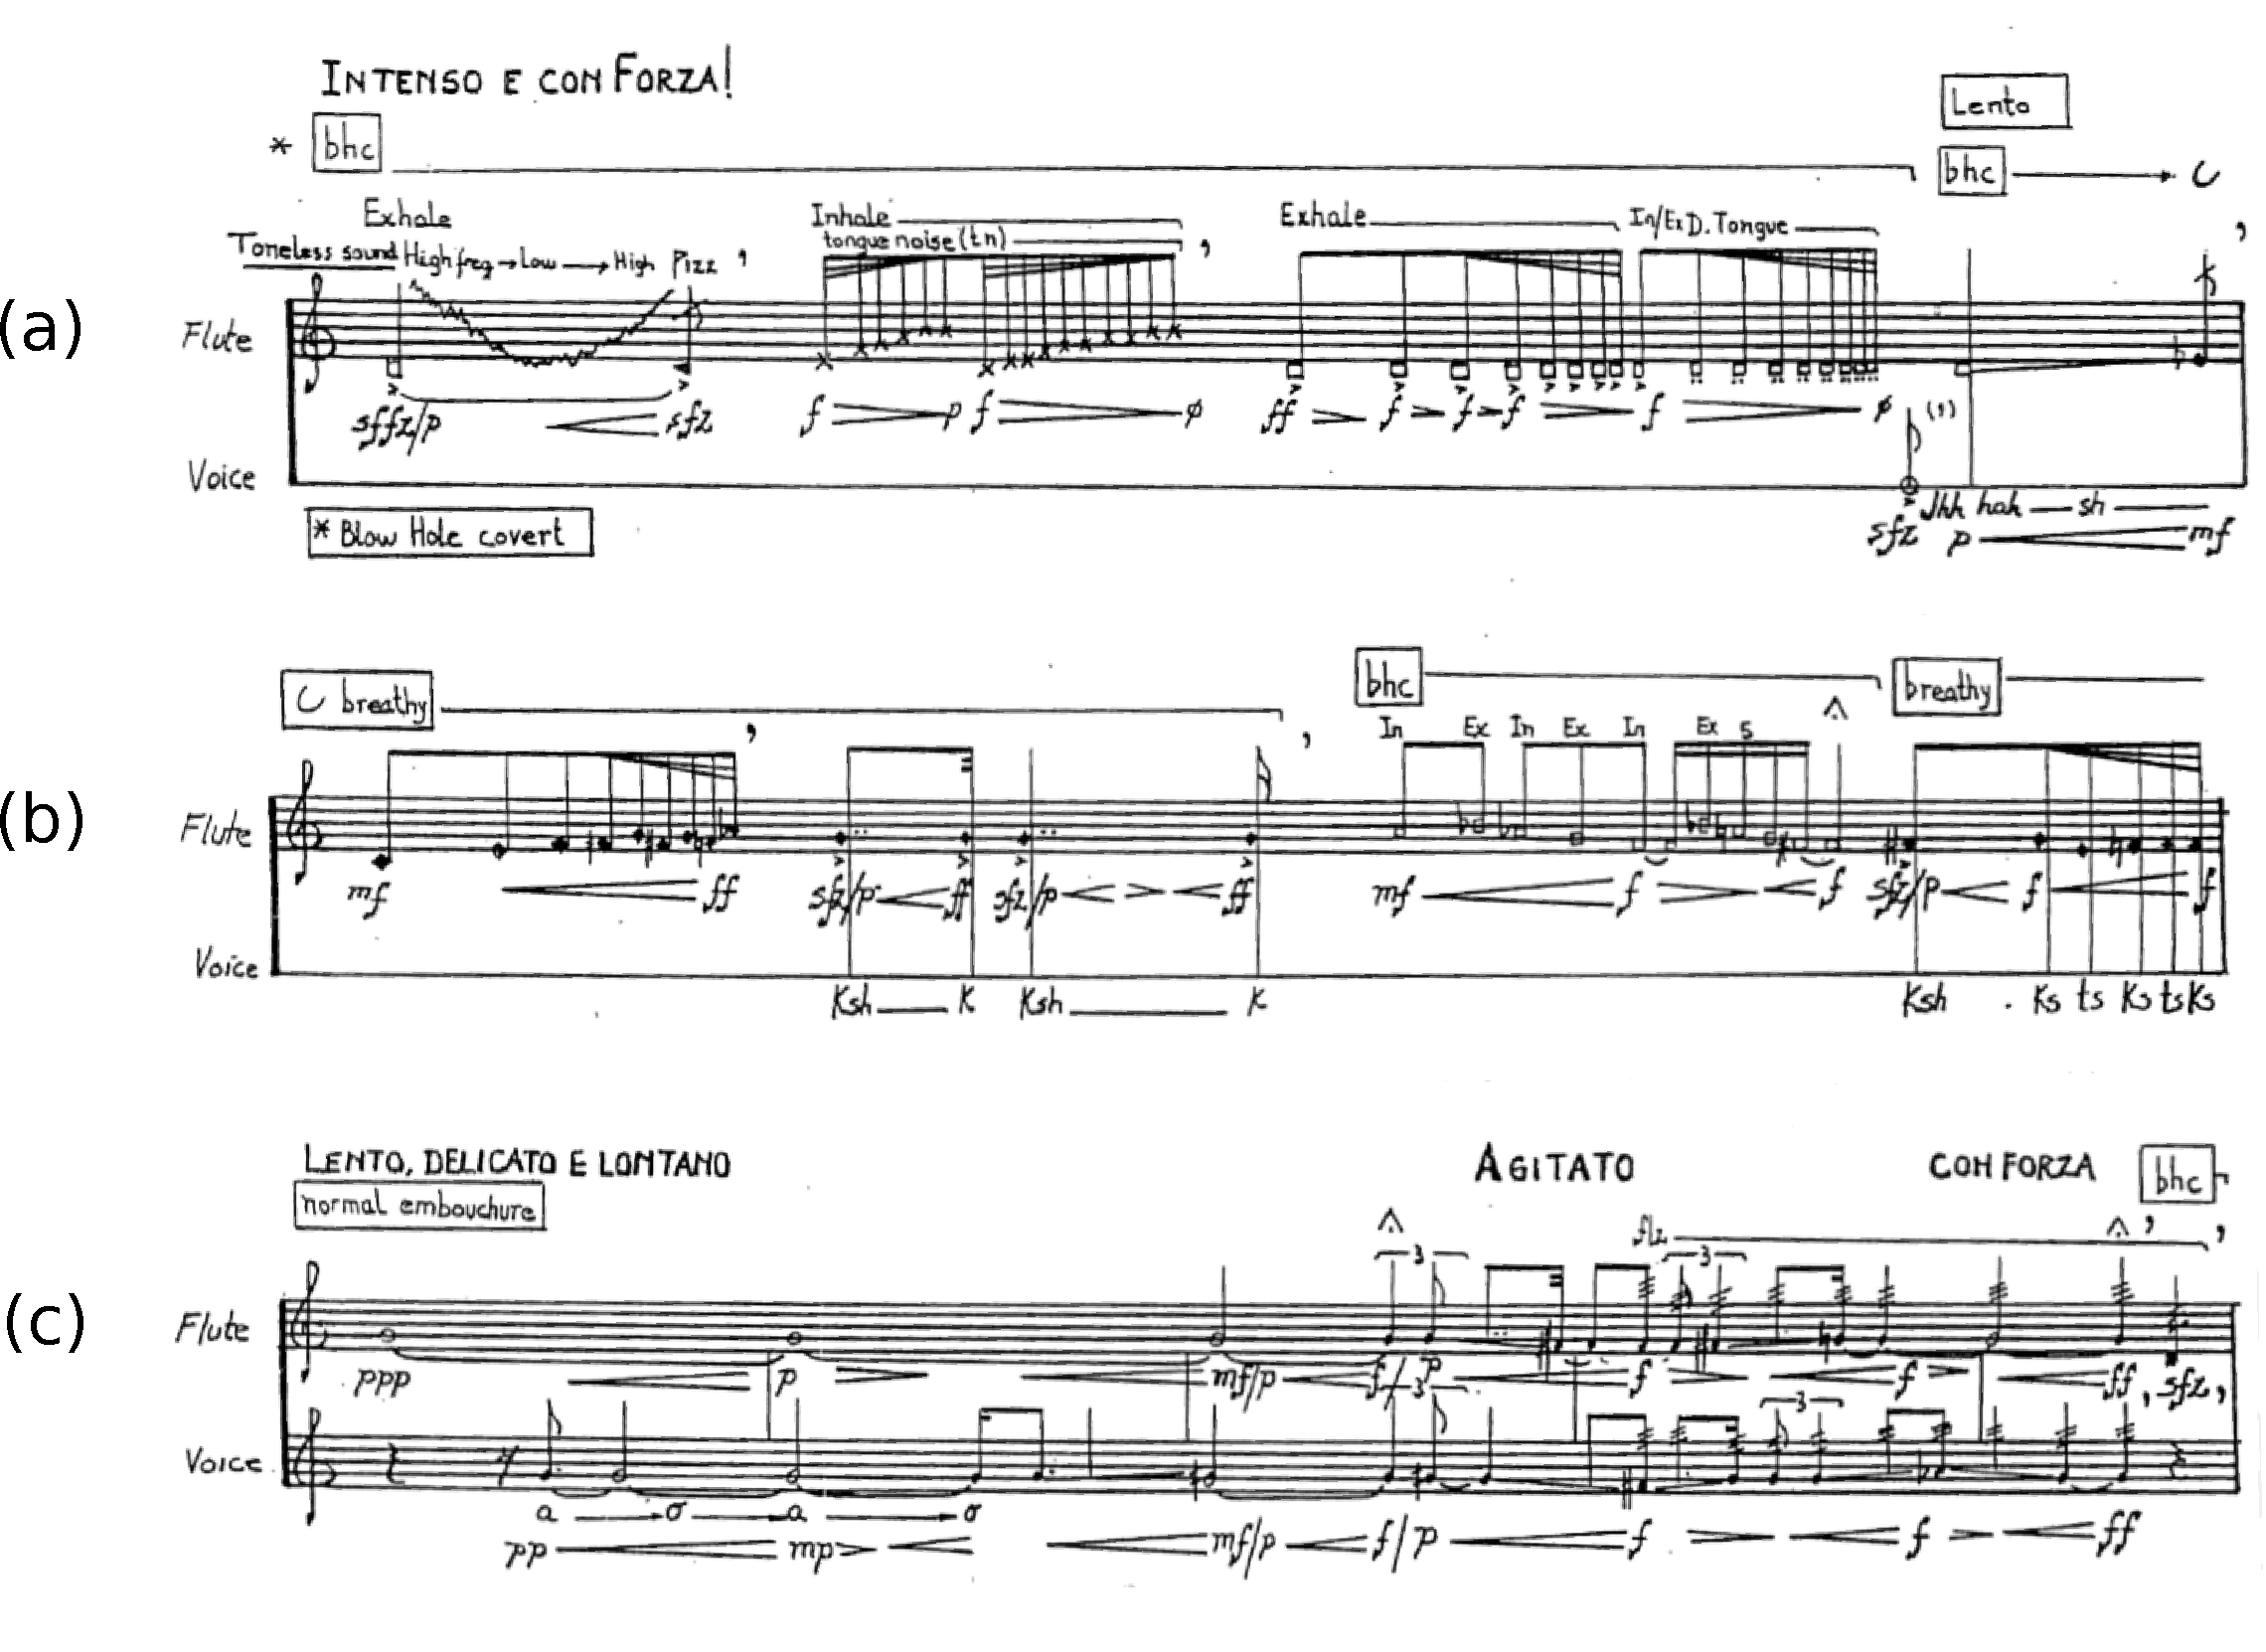
\includegraphics[width=0.9\textwidth]{embocaduras} 
\caption{Notación de las embocaduras se observa en la parte superior de los sistemas. (a) \textit{Blow Hole Covert}. (b) \textit{Breathy Embouchure}. (c) \textit{Normal Embouchure}. Fragmentos extraídos de la partitura de Aliento/Arrugas.}
\label{fig:embocaduras}
\end{center}
\end{figure}

\section{Definición del Problema}
Teniendo en cuenta que la embocadura es un elemento determinante del material sonoro ejecutado perceptible de forma auditiva (Sección \ref{embocadura}), se propone la extracción automática del tipo de embocadura a través del análisis computacional de grabaciones de la obra. 


\subsection{Estrategia de resolución}

Se propone la resolución del problema con un enfoque de reconocimiento de patrones. Se procesa el audio como un \textit{Bag of Frames} a partir del computo de descriptores numéricos. El principal desafío y cometido del presente trabajo es encontrar los descriptores que extraigan las diferencias en la naturaleza sonora y permitan la separación de las embocaduras en el espacio de características. 
\medskip

\subsection{Conjunto de Datos}
\label{datos}
Se cuenta con 5 grabaciones de diferentes intérpretes de la obra Aliento/Arrugas. Los intérpretes son: Pablo Somma, Emma Resmini, Claire Chase, Juan Pablo Quinteros y Ulla Suokko. Los archivos de audio se etiquetaron utilizando el software \textit{Sonic Visualiser} \citep{cannam2010sonic} dividiendo los archivos de audio en 5 clases:

\begin{itemize} 
  \item Silencio.
  \item Silencio con respiración del intérprete. 
  \item Sonido generado con \textit{Blow Hole Covert}.
  \item Sonido generado con \textit{Breathy Embouchure}.
  \item Sonido generado con \textit{Normal Embouchure}.
\end{itemize}

Las grabaciones de Claire Chase y Juan Pablo Quinteros que se obtuvieron para el presente trabajo sufrieron un proceso de compresión con pérdida, por lo que estos datos reciben un tratamiento distinto. No se utilizan para entrenar los algoritmos de clasificación, solo se utilizan como datos de test. Por lo que folds son de la siguiente forma: 

\begin{itemize} 
  \item Cuando la grabación de test es la de Ulla Suokko, Pablo Somma o Emma Resmini, se entrena con las otras dos restantes. Metodología de \textit{Leave One Out} por su demoninación en Inglés.
  \item Por otro lado cuando la grabación de test es de Claire Chase o Juan Pablo Quinteros, el conjunto de entrenamiento esta compuesto por las tres grabaciones sin pérdida (i.e. la de Ulla Suokko, Pablo Somma y Emma Resmini).
\end{itemize}

En lo que sigue se utilizan únicamente las clases asociadas a cada una de las embocaduras. Queda por fuera del alcance de este trabajo, una etapa de pre-procesamiento para la segmentación del audio en fragmentos de actividad de la flauta y silencios (este problema se conocido como \textit{Activity Detection} por su denominación en Inglés). 
\medskip 

MOSTRAR LAS PROPORCIONES DE LAS CLASES! NO SEAS MALO!

\subsection{Extracción de características}
\label{descriptores}
Se enlistan a continuación las características que se evalúan en la extracción automática de embocadura. Además se describe brevemente sus principales atributos.



\subsubsection{Mel-Frequency Cepstral Coefficients (MFCC)} 

Los \textit{Coeficientes Cepstrales de Frecuencia-Mel} fueron introducidos por \cite{davis1980comparison} en la resolución del problema de reconocimiento del hablante a partir de señales de voz (\textit{Speaker Recognition} su denominación en Inglés). Estos coeficientes como características de un sistema de reconocimiento automático del hablante han demostrado tener de los mejores desempeños \citep[Capítulo~14]{quatieri2002discrete}. A partir de ahí han sido utilizados en diversas problemáticas de clasificación que no involucran señales de voz hablada, con buenos resultados también como es el caso de reconocimiento de instrumentos \citep[Capítulo~6]{klapuri2007signal}. Su fortaleza radica en la incorporación del modelado psicoacústico de la audición humana mediante un banco de filtros basados en la escala Mel \citep{stevens1937scale} y la decorrleación que presentan los datos en el dominio de las \textit{quefrencys}, dado por la aplicación de la Transformada Coseno. Son un buen descriptor para la extracción de aspectos tímbricos de la señal.
\medskip

El cómputo de estas características cuenta con las etapas que se enlistan a continuación de manera conceptual: 

\begin{enumerate}
	\item División de la señal en fragmentos mediante enventanado.
	\item Cálculo de la magnitud de la Transformada discreta de Fourier de tiempo corto (STFT).
	\item Fitrado de la señal con banco de filtros Mel.
	\item Cálculo de la energía para cada filtro del banco.
	\item Logaritmo de las energías.
	\item Transformada Coseno de los valores a la salida del Logaritmo.
	\item \textit{Liftrado} de la señal resultante en el dominio de las \textit{quefrencys}, luego de la Transformada Coseno. Determina la cantidad de coeficientes, o en otras palabaras la dimensión del espacio de caracterísitcas.
\end{enumerate}

El cálculo de los coeficientes MFCC tiene los siguientes parámetros determinantes de su desempeño: En primer lugar el largo de las ventanas, que define el compromiso entre resolución temporal y espectral. En segundo lugar la cantidad de filtros del banco de filtros Mel, que se puede pensar como un submuestreo de la resolución espectral ya determinada por el largo del enventanado. Por último el \textit{liftrado} de la señal a la salida de la Transformada Coseno que determina la cantidad de coeficientes efectivos previos al clasificador.
\medskip


\subsubsection{Linear Prediction Coefficients (LPC)}

La técnica de análisis de señales de tiempo discreto por predicción lineal, tiene su aplicación en diversas áreas del conocimiento. Es parte de un problema más general denominado \textit{identificación de sistemas} desarrollado en el área de control para el análisis de sistemas dinámicos. Supone que la señal de análisis es la salida $s[n]$ de un sistema lineal con entrada $u[n]$. Su fortaleza y versatilidad radica en la estimación de parámetros del sistema lineal que define el problema. 
\medskip

Su enunciado más general modela la señal de análisis como un proceso \textit{Auto-Regresivo de Media Móvil (ARMA)} \citep{makhoul1975linear}. En otras palabras, supone que la muestra actual de la señal de análisis puede ser expresada como una combinación lineal de las muetras pasadas de la salida, y la muestra actual y pasadas de la entrada: 

\begin{equation}
\label{eq:arma}
s[n]=-\sum_{k=1}^p a_ks[n-k]+G\sum_{l=0}^p b_lu[n-l]
\end{equation}

Ha sido utilizado para la resolución de problemas con señales de audio, en particular existe mucha literatura al respecto con la voz humana. Para voz hablada es de los métodos más poderosos, con diversas aplicaciones. La importancia de este método se basa tanto en la precisión de la estimación de parámetros del modelo de mecanismo de producción de voz, como en su relativo bajo costo computacional \citep[Capítulos~3 y 9]{rabiner1978digital}. 
\medskip

Alineado con la utilización de LPC en problemas de señales de voz, se supone que es suficiente un modelo todo-polos para la extracción de características en el presente trabajo. De forma matemática a partir de la Ecuación \ref{eq:arma} se escribe como $b_l=0$ con $l=1...p$. Los parámetros relevantes en el computo del descriptor son entonces, en primer lugar $p$ asociado a la cantidad de polos del modelo $AR$ y por otro lado el largo de las ventanas de análisis. Componiendo el vector de características por los coeficientes $a_k$ con $k=1...p$ (ver Ecuación \ref{eq:arma}).

\subsubsection{Conjunto de características Espectrales y Armónicas} 
Se genera un vector compuesto por 5 características acústicas uni-dimensionales, para evaluación del desempeño en la extracción de embocadura. Entre los descriptores se optaron por 4 medidas espectrales y una medida de armónica de la señal de análisis, según la taxonomía de \textit{features} acústicos propuesta en el libro de \cite{klapuri2007signal}. Las características son: 

\begin{itemize}
	\item Voicing: Es una medida de periodicidad de la señal. Es el \textit{feature} armónico del conjunto. Generalmente el Voicing se encuentra embebido en los algoritmos de extracción de pitch. En particular para el presente trabajo se computa como en la referencia: \cite{de2002yin}.   
	\item Zero-Crossing Rate: Mide la cantidad de cruces por cero de la señal. Si bien es calculado en el dominio del tiempo, es una medida del contenido de alta frecuencia.
	\item Roll-off: Es el valor de frecuencia para el que la energia espectral acumulada supera una fracción denominada $\lambda$. En general $\lambda$ se elige $95\%$ o $85\%$. 
	\item Centroid: Es el promedio en los bins de frecuencia ponderado por los valores de magnitud del espectro. Se puede pensar como el centro de masa en el espectro. 
	\item Bandwidth: Es una medida de la dispersión spectral con respecto al centroide.
\end{itemize}

En todas las medidas acústicas recién mencionada es de relevancia la elección del largo de la ventana análisis, que define el compromiso entre estacionariedad de la señal y resolución en frecuencia.

\subsubsection{Octave-based Spectral Contrast (SC)}

El \textit{Contraste Espectral por Octavas} fue desarrollado en el trabajo publicado por \cite{jiang2002music}. Tiene como cometido ser una medida de las características relativas del espectro de la señal de análisis. Extrae la diferencia entre la prominencia de los picos en el espectro y los valles en cada octava de análisis por separado. Ha tenido buenos resultados en el problema de clasificación de estilo musical.
\medskip

El cómputo de estas características tiene las siguientes etapas, que se enuncian de forma conceptual:

\begin{enumerate}
	\item División de la señal en fragmentos mediante enventanado.
	\item Cálculo de la magnitud de la Transformada discreta de Fourier de tiempo corto (STFT).
	\item Fitrado de la señal con banco de filtros por octava.
	\item Cálculo de la diferencia entre la energía en un entorno de los picos y de los valles en cada una de las octavas.
	\item Logaritmo de las diferencias del paso anterior.
	\item Transformada \textit{Karhunen-Loeve} para representación de las características en base ortonormal y decorrelación entre las dimensiones.
\end{enumerate}

A diferencia de \textit{MFCC} y \textit{LPC} que realizan un promediado de la información espectral, estos descriptores extraen la información relativa, mediante la comparación de picos y valles por octava. Los parámetros relevantes son en primer lugar el largo de la ventana de análsis, el entorno de los picos y valles denominado $\alpha$ en la literatura, y por último el número de octavas. 

%\subsection{Análisis de la naturaleza acústica del problema}
%
%Las tres embocaduras utilizadas en Aliento/Arrugas tienen como propósito generar variación en el material sonoro de la pieza. Los parámetros acústicos que 
%
%\subsubsection{Resultados}
%Para el cálculo se utilizan ventanas de análisis de $23ms$ y saltos del $50\%$ del largo de la ventana. Se dejaron afuera del análisis las clases: \textit{Silencio} y \textit{Silencio con respiración del intérprete}.
%\medskip
%
%A continuación en la Figuras \ref{fig:histogramas_artista} y \ref{fig:comparative} se observa el espacio de características con distinción por clase para los diferentes intérpretes. Se puede observar que la \textit{Normal Embrochure} es separable frente al resto con estos cálculos. No es así el caso de las embocaduras \textit{Blow Hole Covered} y \textit{Breathy Embrocuhre}.
%
%\begin{figure}[H]
%\begin{center}
%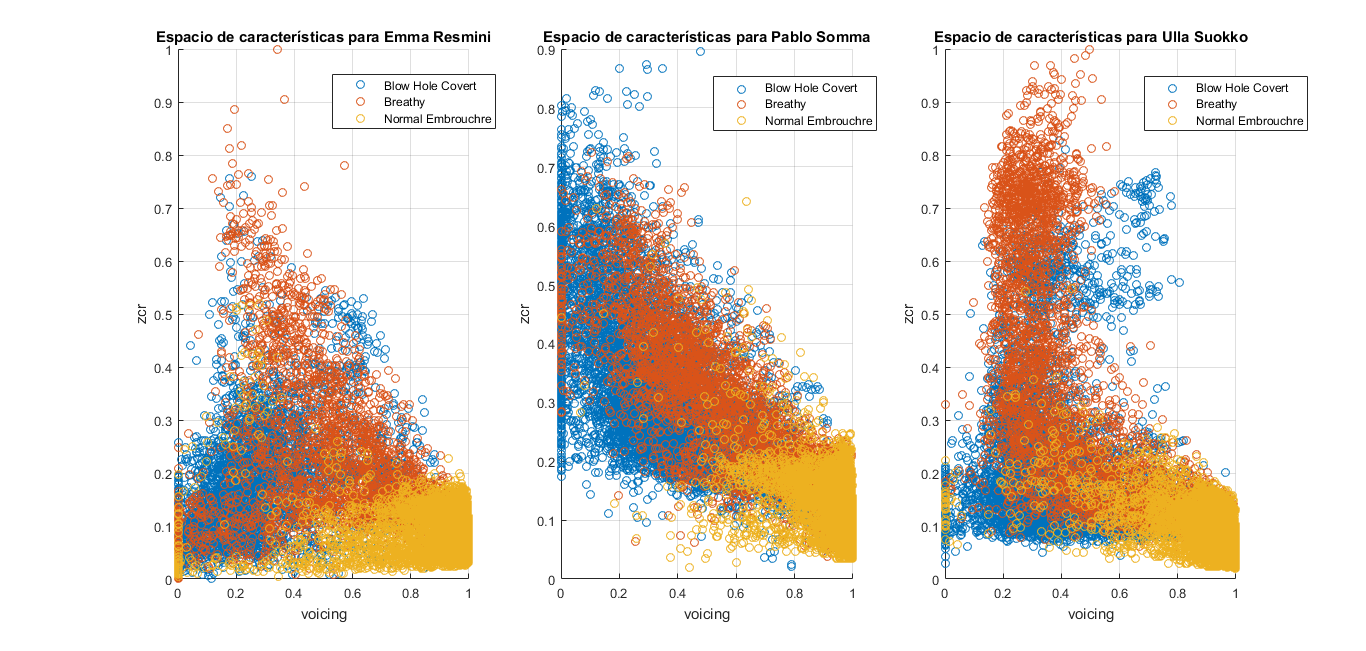
\includegraphics[width=1\textwidth]{histograms_artist} 
%\caption{Espacio de características etiquetado por clases para cada uno de las interpretaciones.}
%\label{fig:histogramas_artista}
%\end{center}
%\end{figure}
%
%\begin{figure}[H]
%\begin{center}
%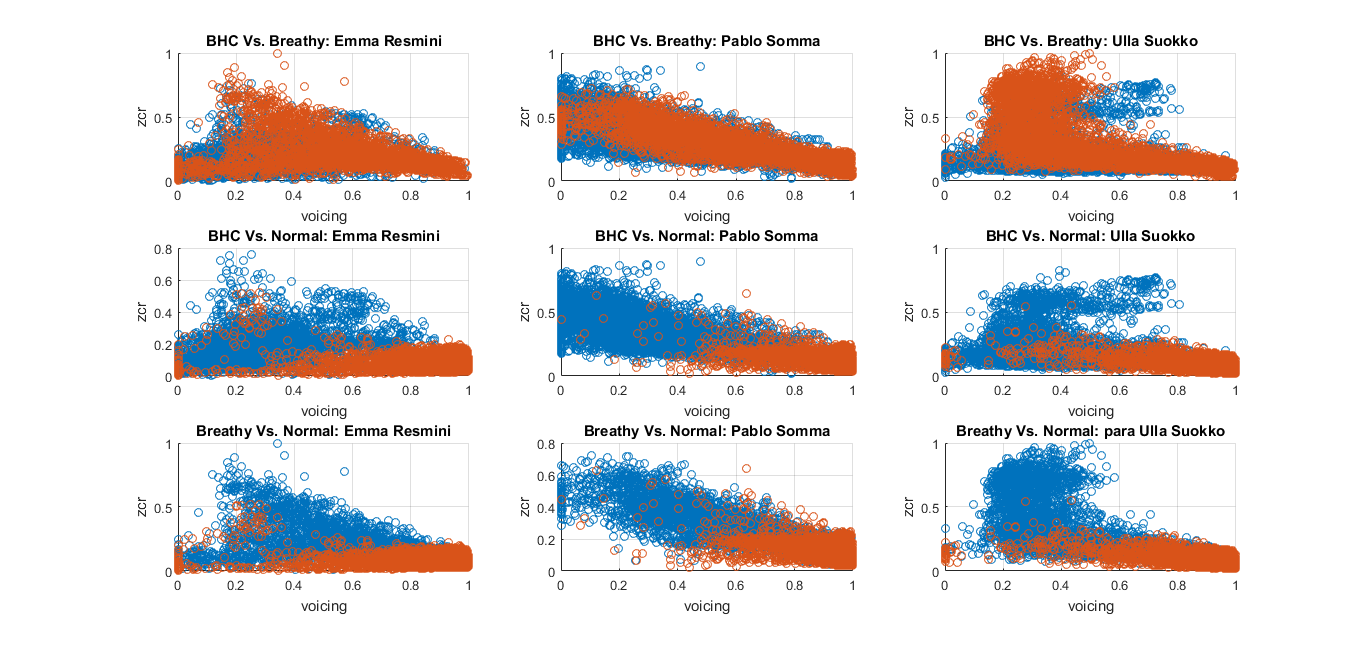
\includegraphics[width=1\textwidth]{comparative} 
%\caption{Comparación clase vs. clase en el espacio de características.}
%\label{fig:comparative}
%\end{center}
%\end{figure}
%
%\newpage
%
%
%Se observa además en las Figuras \ref{fig:bhc_features}, \ref{fig:breathyemb_features} y \ref{fig:normalemb_features} el comportamiento temporal de las características \textit{Voicing} y \textit{Zero-Crossing Rate} superpuestas con el espectrograma, para tres fragmentos de la interpretación de Emma Resmini. Corresponden a \textit{Blow Hole Covered}, \textit{Breathy Embrochure} y \textit{Normal Embrochure} respectivamente. Se corrobora lo dicho anteriormente sobre la separabilidad entre clases.
%
%\begin{figure}[H]
%\begin{center}
%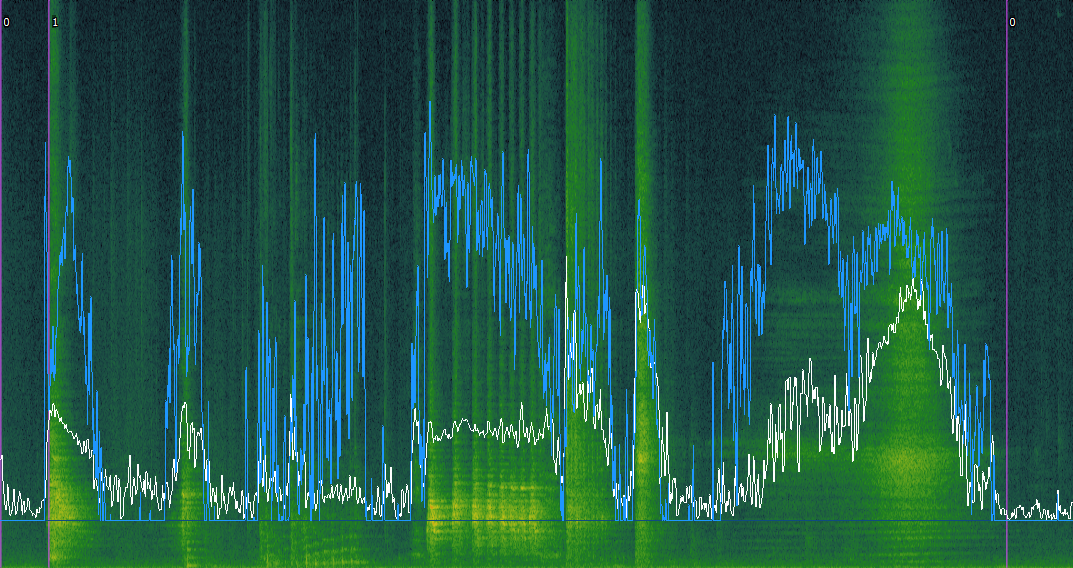
\includegraphics[width=1\textwidth]{bhc_features} 
%\caption{Visualización de un fragmento de la interpretación de Emma Resmini con embocadura \textit{Blow Hole Covered}. Se observa en celeste el \textit{Voicing} y en blanco \textit{Zero-Crossing Rate}.}
%\label{fig:bhc_features}
%\end{center}
%\end{figure}
%
%
%\begin{figure}[H]
%\begin{center}
%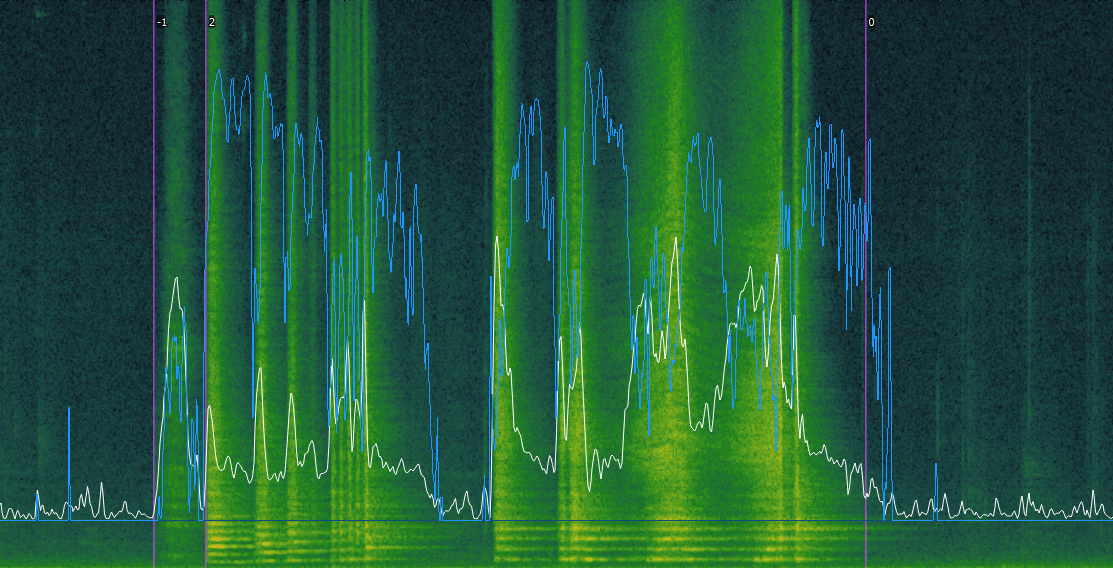
\includegraphics[width=1\textwidth]{breathyemb_features} 
%\caption{Visualización de un fragmento de la interpretación de Emma Resmini con embocadura \textit{Breathy Embrochure}. Se observa en celeste el \textit{Voicing} y en blanco \textit{Zero-Crossing Rate}.}
%\label{fig:breathyemb_features}
%\end{center}
%\end{figure}
%
%


   
\section{Experimentos}

Se evalúa la capacidad de los descriptores presentados en la Sección \ref{descriptores} en la separación de embocaduras. Para esto se utilizan tres clasificadores distintos para minimizar el bías que pueda existir entre los datos y un algoritmo en particular. Se trabaja con los algoritmos: \textit{Random Forest (trees=10)}, \textit{Support Vector Machine (kernel lineal)} y \textit{K-Nearest Neighbors (k=10)}. En todos los casos se utilizan los parámetros por defecto ya que no es objetivo de este trabajo encontrar los valores óptimos de clasificación. La implementación se realiza mediante el módulo de \textit{Python} llamado \textit{Scikit Learn} \citep{pedregosa2011scikit}. En todos los casos los datos son preprocesados de manera de centrar en cero y escalar la varianza a uno, previo al clasificador.
\medskip

Todos los experimentos se realizan con \textit{5-fold cross validation} donde los folds son las diferentes interpretaciones de la pieza musical, como se detalla en la Sección \ref{datos}. De esta forma se asegura que frames provenientes de la misma grabación no sean usados para train y test en un mismo experimento.
\medskip

\subsection{Primer experimento: Mejor descriptor para extracción de embocadura}

El propósito es cuantificar el poder de separación de las características y determinar cual tiene el mejor desempeño. Para tener una noción general del comportamiento de los descriptores, en todos los casos se utiliza más de una combinación de parámetros. Se eligieron de forma que sea suficiente para descartar los de menor desempeño. A continuación se enlistan los parámetros utilizados en cada caso.

\begin{itemize}
	\item Característcas Espectrales y Armónicas: Se varían los largos de ventana y saltos de la siguiente forma (se detallan respectivamente): (a) $11ms$ y $50\%$ de salto (256-128 muestras), (b) $23ms$ y $50\%$  (1024-512 muestras) y por último (c) $46ms$ y $50\%$  (2048-1024 muestras). En todos los casos anteriores se utilizó: 
	\begin{itemize}
		\item Voicing: Número de retardos: 250 muestras.
		\item Roll-off: $\lambda=85\%$
		\item Centroid, Bandwith y Zero-Crossing Rate: quedan definidos por el largo de la ventana de análisis y el salto.
	\end{itemize}
	\item MFCC: Se computan con ventana de análisis de $23ms$ y salto del $50\%$, 40 bandas Mel y se liftra la señal para obtener: (a) 20 coeficientes, (b) 30 coeficientes y (c) 40 coeficientes.
	\item LPC: Se computan con ventana de análisis de $23ms$ y salto del $50\%$ y numero de polos: (a) 10, (b) 20 y (c) 40.
	\item SC: Se computan con ventana de análisis de $23ms$ y salto del $50\%$ y numero de bandas: (a) 3 y (b) 6.
\end{itemize}

\subsection{Resultados}

En lo que sigue se muestra el resultado del desempeño de los descriptores detallados en la Sección \ref{descriptores} para la extracción del tipo de embocadura.
\medskip

\begin{figure}[H]
\begin{center}
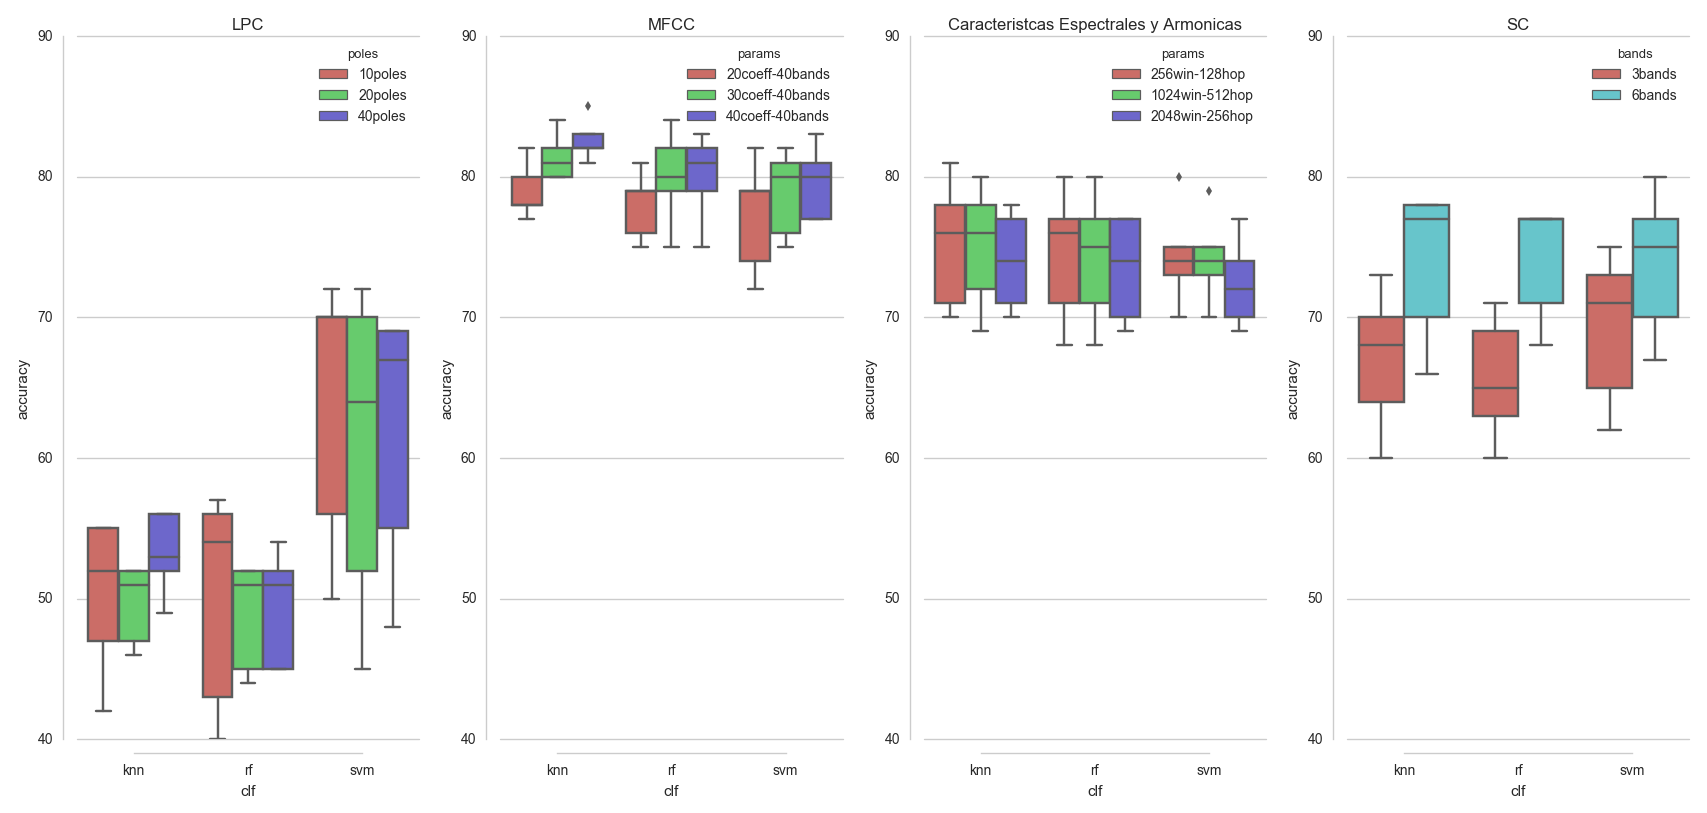
\includegraphics[width=1\textwidth]{exp1_comparacion} 
\caption{Boxplot para el accuracy de los algoritmos de clasificación. Se muestra los resultados de forma independiente por algoritmo de clasificación y según los parámetros de las características}
\label{fig:exp1_comparacion}
\end{center}
\end{figure}

\begin{figure}[H]
\begin{center}
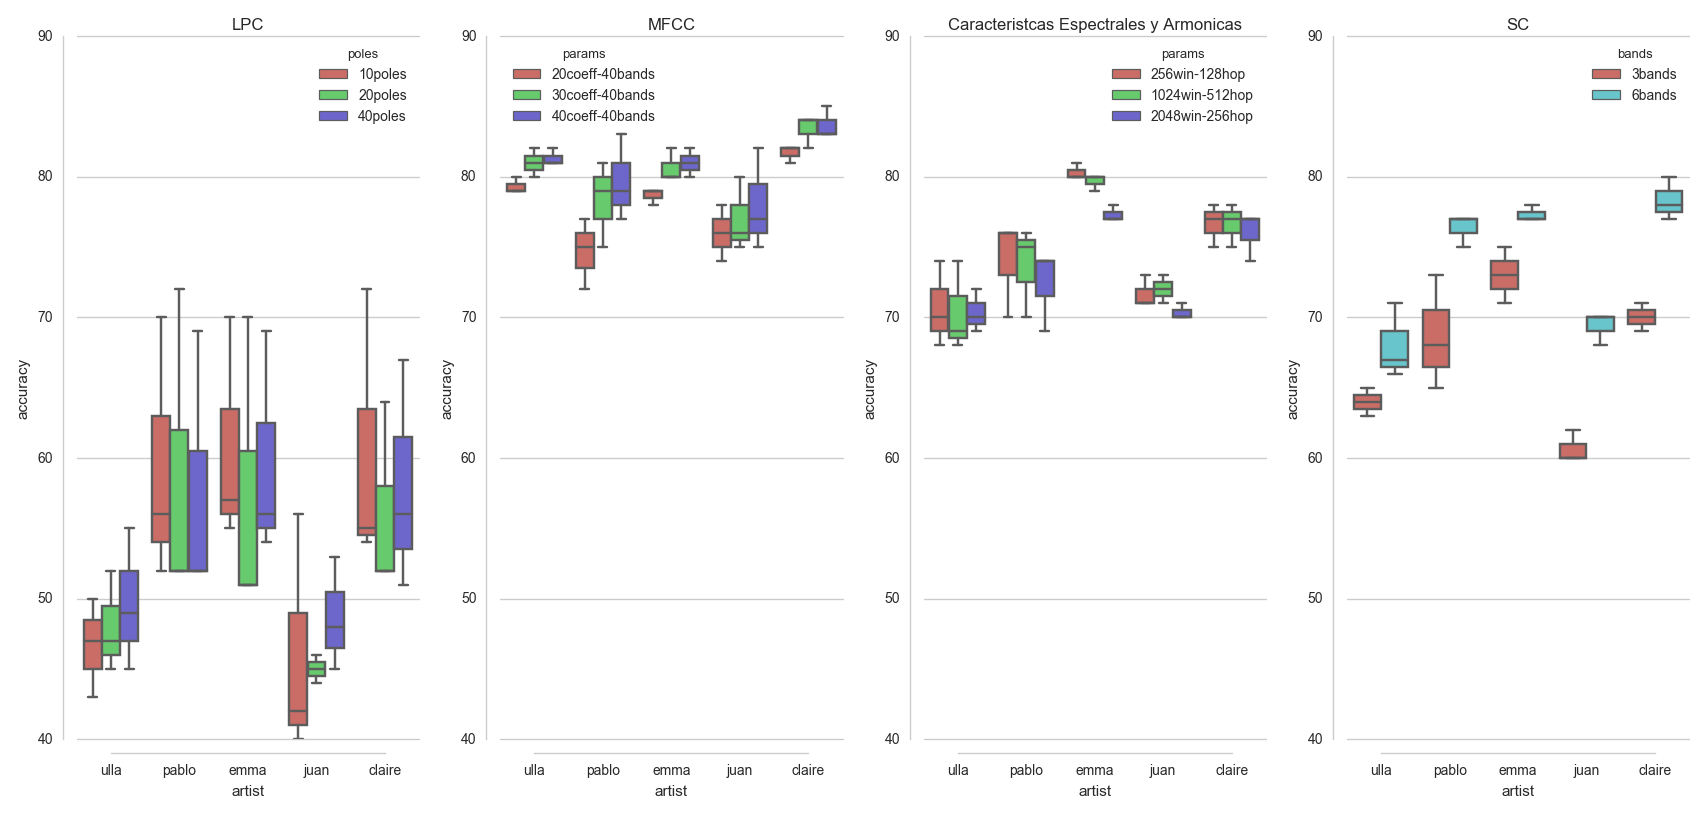
\includegraphics[width=1\textwidth]{exp1_artista} 
\caption{Boxplot para el accuracy de los algoritmos de clasificación. Se muestra los resultados de forma independiente por artista (fold) y según los parámetros de las características.}
\label{fig:exp1_artista}
\end{center}
\end{figure}

PRIMERO MOSTRAR COMPARACIÓN ENTRE FEATURES!!!!
LPC: Carece de modelado fisico del problema que pueda validar y dar pistas de los parámetros relevantes
SPECTRAL AND HARMONIC FEATURES: redundancia!!!!!!! algún approach de decorrelación podría ayudar, pero hablar de la importancia del knowledge!
Spectral contrast: anda bien y a priori podría ser mas suitable para el problema, pero debido a q mfcc funcionó mejor se sigue adelante

\begin{figure}[H]
\begin{center}
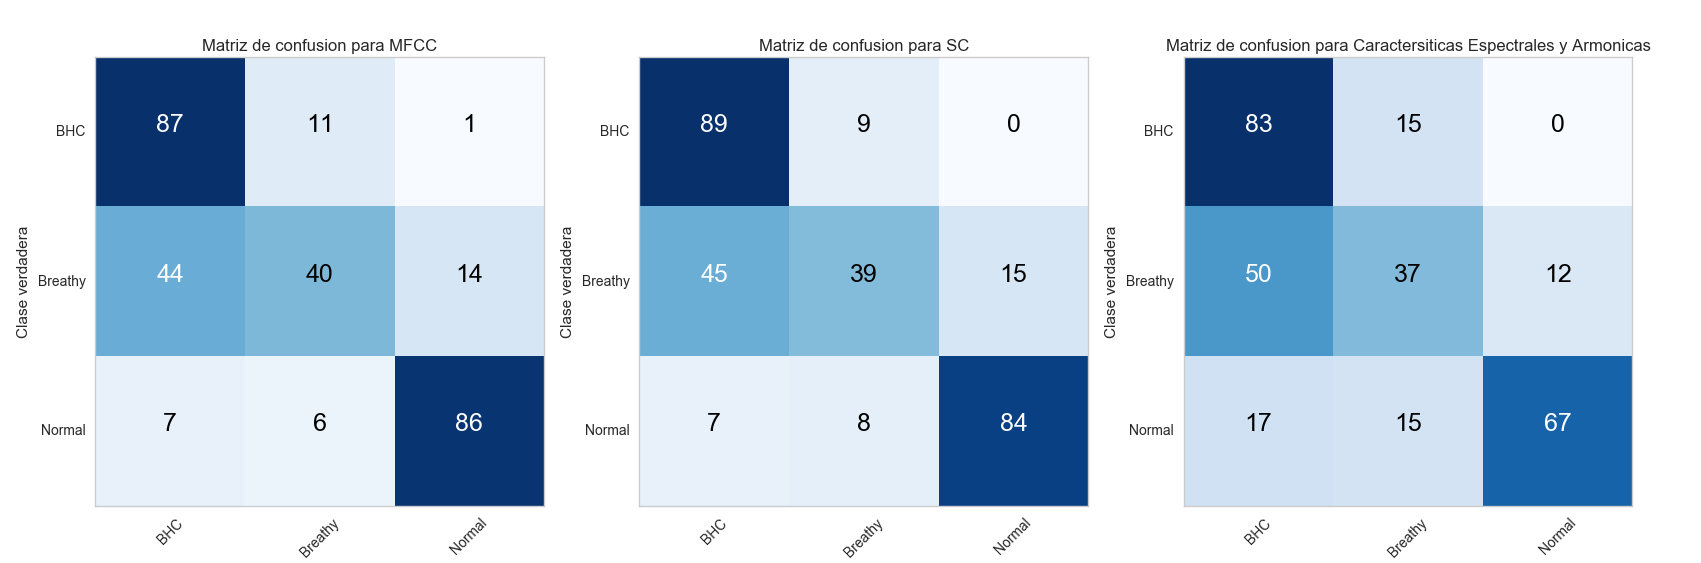
\includegraphics[width=1\textwidth]{exp1_confusion} 
\caption{Matrices de confusión para las características MFCC, SC, y Características Espectrales y Armónicas de izquierda a derecha respectivamente. Para todos los casos el algoritmo de clasificación es KNN.}
\label{fig:exp1_confusion}
\end{center}
\end{figure}

\subsection{Segundo experimento: Blow Hole Covert Vs. Breathy}

\begin{figure}[H]
\begin{center}
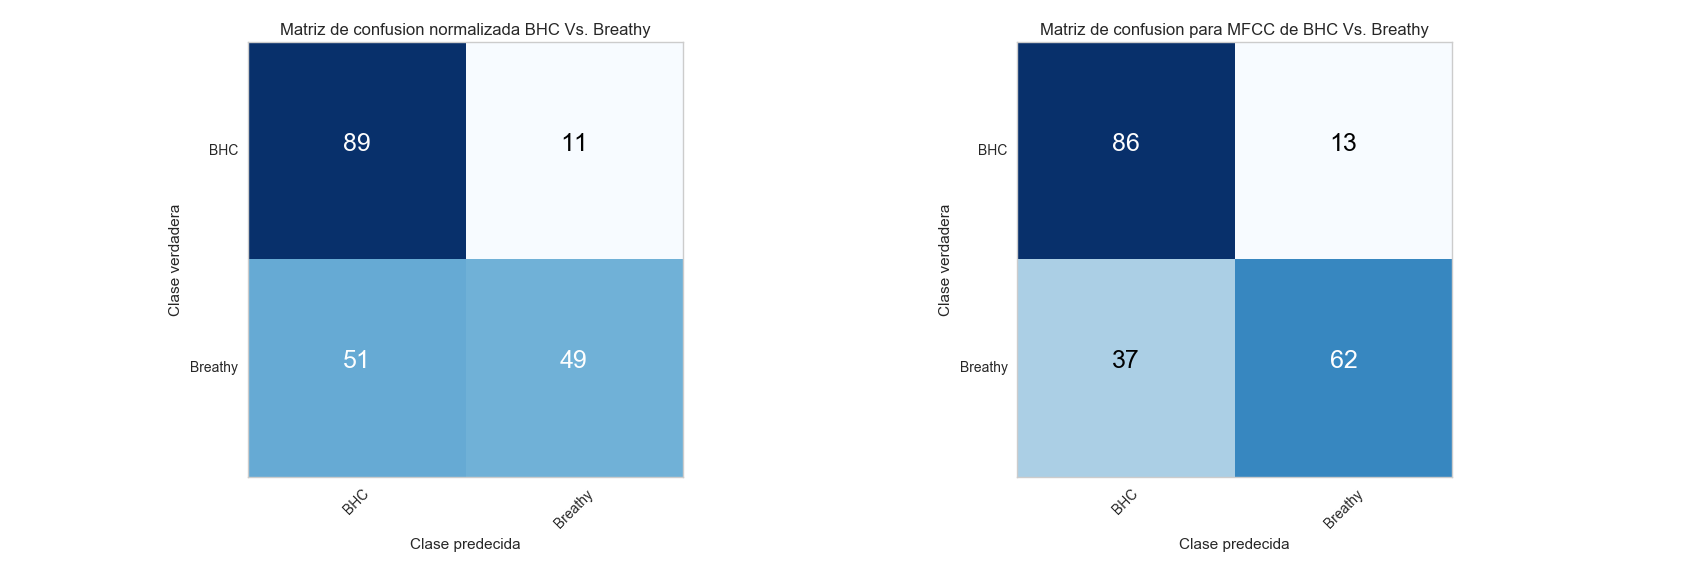
\includegraphics[width=1\textwidth]{exp1_confusion2} 
\caption{Matrices de confusión para las clases \textit{BHC} Vs. \textit{Breathy} generadas con características MFCC y el clasificador KNN.}
\label{fig:exp1_confusion2}
\end{center}
\end{figure}

Y ME QUEDO CON MFCC PORQUE ES UN FIERRO
PRESENTA DOS PROBLEMÁTICAS: 
NINGÚN FEATURE LOGRA SEPARAR BREATHY VS. BHC: se prueba solo con esas dos clases y mfcc20 (por simplicidad para el computo y clasificador) 
-LA CLASE TONAL QUE SERÍA LA MÁS SEPARABLE PRESENTA CONFUSIÓN QUE PODRÍA EVITARSE CON EL VOICING (?) : MFCC es un fierro pero apriori no tiene porque utilizar la información de periodicidad propiamente dicha. Parámetro relevante en la separación de estos tres tipos de embocadura. Se agrega voicing tipo yin \cite{de2002yin}
 
\subsection{Tercer Experimento: Refinamiento de MFCC}
Compromiso resolución en frecuencia resolución temporal




Se identifica nuevamente el problema en la separación

Comparar confusión entre 2x2 y 3x3 en la separación de BHC y BREATHY

Discusión de agregar voicing, ver como mejora la matriz de confusión 

Hablar que la confusión puede ser por articulaciones similares con distinta embocadura, mirar mariana stratta

\subsubsection{}


\section{Trabajo a futuro}

\begin{itemize} 
  \item Segmentación de audio, umbralizando los silencios y las respiraciones 
  \item Salir del bag of frames, para utilizar la redundancia temporal
  \item Dejar Planteado el sistema completo! diagrama de bloques!
\end{itemize}
%----------------------------------------------------------------------------------------
%	BIBLIOGRAPHY
%----------------------------------------------------------------------------------------


\newpage
\bibliographystyle{apalike}
\bibliography{biblio}


%----------------------------------------------------------------------------------------
\end{document}


